\documentclass[11pt,a4paper]{article}

\usepackage[utf8]{inputenc}
\usepackage[T1]{fontenc}
\usepackage{amsmath,amssymb,amsfonts}
\usepackage{graphicx}
\usepackage{booktabs}
\usepackage{xcolor}
\usepackage{hyperref}
\usepackage{geometry}
\usepackage{authblk}
\usepackage{listings}
\usepackage{microtype}
\geometry{margin=1in}
\hypersetup{
  colorlinks=true,
  linkcolor=blue,
  citecolor=blue,
  urlcolor=blue,
}
\lstset{
  basicstyle=\ttfamily\small,
  breaklines=true,
  frame=single,
  numbers=none,
}

\title{\textbf{flatmem}: A Constant-RAM Content-Addressable Memory Substrate \\
       for Digital Organisms and Artificial Life Agents}

\author{Prince Siddhpara}
\affil{Mura ALife Labs}
\date{May 2026}

\begin{document}

\maketitle

\begin{abstract}
We present \texttt{flatmem}, a constant-RAM content-addressable memory
substrate for online-learning digital organisms. The architecture integrates
five mathematical primitives---Sparse Distributed Memory (SDM)
\cite{kanerva1988sparse}, Vector Symbolic Architecture (VSA) role-binding
\cite{plate1995holographic,kanerva2009hyperdimensional}, computed-identity
keys, read-time mean-removal \cite{mu2017all}, and traffic-class bank
separation---into a single substrate whose total bytes are \emph{fixed}
regardless of how much information is written.  A trained instance occupies
192 MB of substrate carrying co-occurrence statistics, IS-A taxonomy,
sensory grounding, verb-rotor arithmetic, transition probabilities, and
classification labels for a natural-language plus vision organism;  full
inference RAM is 233 MB.  We empirically demonstrate constant-RAM behavior
up to 100K text exposures (vocabulary of 19{,}411 words), substrate-flatness
through cross-modal training, modality-blind extension to a vision channel
(90\% test accuracy on 8$\times$8 digit classification), and---most
critically---catastrophic-forgetting-free continual learning: 5 original
facts retained with $100\%$ recall through 5{,}000+ distractor writes
spanning four different channels.  We argue \texttt{flatmem} is the
universal flat-memory primitive for Artificial Life simulations, embedded
agents, and any system that needs lifelong learning within a bounded RAM
budget.  Code is open-source under MIT license at
\url{https://github.com/HitoshiFTW/Flatmem-Mura-ALife-Labs} and installable
via \texttt{pip install flatmem}.
\end{abstract}

\section{Introduction}
\label{sec:intro}

Modern machine learning systems scale memory with data.  Embedding tables
in language models grow with vocabulary; replay buffers grow with corpus
size; vector databases grow linearly with stored items.  Biological brains
do neither.  An adult human cortex contains roughly $86 \times 10^9$ neurons
fixed from development; a lifetime of experience is encoded in the
\emph{strengths} of synaptic connections within that fixed matrix, not in
newly allocated storage.  This gap has practical consequences for
online-learning systems in robotics, multi-agent simulations, and edge
deployment, where unbounded growth is unacceptable.

Existing approaches sit at extremes.  Static word-embedding tables
(\textsc{word2vec}, \textsc{GloVe}) require an entry per token---memory
$\Theta(|V|)$ in vocabulary $|V|$.  Vector databases inherit this growth.
Neural networks compress vocabulary into hidden layers but suffer
catastrophic forgetting under sequential training
\cite{mccloskey1989catastrophic,french1999catastrophic} without expensive
remediation (replay buffers, LoRA, full retraining).  Sparse Distributed
Memory (Kanerva 1988 \cite{kanerva1988sparse}) provides a biologically
grounded fixed-capacity substrate but, in its classical form, supports only
single-channel autoassociative recall.

This work proposes a different design point.  The substrate is a
fixed-size counter bank.  Knowledge is \emph{superposed} across many
cells; each cell participates in many memories.  Identity is
\emph{computed} from input strings or vectors rather than looked up in a
table.  Recall is \emph{reconstructive}---lossy and gist-based, like human
memory.  The result is a substrate that:

\begin{itemize}
  \item Learns online (single-write per fact, no gradients).
  \item Never forgets catastrophically (additive superposition).
  \item Has bounded RAM at any data volume.
  \item Runs on a laptop CPU (CPU-only inference, no GPU required).
  \item Hosts multiple channels in one substrate (text, taxonomy, sensory,
        arithmetic, transitions, classification).
  \item Is modality-blind (text and pixels coexist).
\end{itemize}

\section{Background}
\label{sec:background}

\subsection{Sparse Distributed Memory}
Kanerva (1988) \cite{kanerva1988sparse} introduced SDM as a mathematical
model of cerebellar function, building on Marr \cite{marr1969cerebellum}
and Albus \cite{albus1971theory}.  The substrate is a bank of $M$ hard
locations with random binary addresses;  writing activates the subset of
locations within Hamming radius $r$ of the query;  reading averages the
contents of activated locations.  Frady and Sommer \cite{frady2019robust}
extended SDM to complex phasor space (Threshold Phasor Associative Memory,
TPAM), gaining native support for continuous quantities and significantly
higher capacity than binary SDM.

\subsection{Vector Symbolic Architectures}
Plate's Holographic Reduced Representations (HRR) \cite{plate1995holographic}
and Kanerva's Spatter Codes \cite{kanerva2009hyperdimensional} showed that
structured data (trees, graphs, key-value bundles) can be encoded as flat
vectors via \emph{binding} (typically circular convolution or
component-wise multiplication) and \emph{bundling} (superposition).  Frady
et al.\ Resonator Networks \cite{frady2020resonator} provide efficient
factorization: iterative inference decomposes superposed bound structures
in $O(\log V)$ operations.

\subsection{Common-direction removal}
Arora and colleagues \cite{mu2017all} observed that pre-trained word
embeddings share a dominant ``common discourse'' direction that suppresses
semantic discrimination.  Removing the top principal components
(``all-but-the-top'') dramatically improves retrieval.  The technique is
presented as a static post-processing step for fixed embedding tables.

\subsection{Hyperdimensional Computing in Artificial Life}
Yilmaz \cite{yilmaz2015symbolic} applied VSA-based reservoir computing to
cellular automata.  Ultra-lightweight edge robotics increasingly leverages
VSA for resource-constrained sensorimotor integration.  Modern Hopfield
networks \cite{krotov2016dense} explore high-capacity associative memory
under adversarial conditions.

\section{Architecture}
\label{sec:arch}

\subsection{Notation}
We work in complex-valued phasor space.  A hypervector (HV) is a vector in
$\mathbb{C}^d$ where each component has unit magnitude ($|h_j| = 1$).  The
default dimension is $d = 512$.  Similarity is the normalized real-part
inner product:
\[
  \cos(a, b) = \frac{\operatorname{Re}\langle a, b \rangle}{d}.
\]
The element-wise complex multiplication $a \odot b$ is the VSA \emph{bind}
operation;  componentwise unit-phasor renormalization is denoted
$\operatorname{renorm}(\cdot)$.

\subsection{Computed identity}
Item identity is not stored.  For a string $w$, the HV is computed as
\begin{align}
  \mathrm{key}(w) = \operatorname{renorm}\!\Big(
    \!\!\sum_{tg \in \mathrm{trigrams}(\#w\#)} P(tg)
    \;+\; \alpha \cdot P(\mathrm{WORD}{:}w)
  \Big),
\end{align}
where $P(\cdot)$ is a seeded random phasor projection
$P(\mathrm{tag}) = \exp(i \cdot \mathrm{uniform}(-\pi, \pi)_d)$ with
$\mathrm{seed} = \mathrm{SHA{-}256}(\mathrm{tag})$.  Char-trigrams give
morphological similarity for out-of-vocabulary inputs;  the whole-word
phasor weight $\alpha = 4$ ensures distinct strings have orthogonal keys
regardless of character overlap.  Empirically, $\cos(\mathrm{key}(\text{little}),
\mathrm{key}(\text{litttle}))$ drops from $0.85$ (trigrams only) to $0.09$
with $\alpha = 4$.  \textbf{Per-item storage: zero bytes.}

\subsection{Sparse Distributed Memory substrate}
The substrate is two arrays: hard-location addresses
$H \in \mathbb{C}^{M \times d}$ (fixed random unit phasors, regenerable
from seed) and learned counters $C \in \mathbb{C}^{M \times d}$ (initialized
to zero, written via Hebbian accumulation).  We use the conjugate
$H^* = \overline{H}$ for similarity computation.

\textbf{Write:}
\begin{align}
  \mathrm{activate}(\mathrm{addr})
    &= \mathrm{top\text{-}k}_{m \in [0, M)}\,
       \operatorname{Re}\langle H^*[m], \mathrm{addr} \rangle, \\
  C[\mathrm{activate}(\mathrm{addr})] &\mathrel{+}= \mathrm{data}.
\end{align}

\textbf{Read:}
\begin{align}
  \mathrm{read}(\mathrm{addr}) = \operatorname{renorm}\Big(
    \!\!\sum_{m \in \mathrm{activate}(\mathrm{addr})} C[m]
  \Big).
\end{align}

Total substrate bytes: $2 \cdot M \cdot d \cdot 8$ (complex64).  With
$M = 16{,}384$, $d = 512$, $k = 64$ this is 128 MB per bank.  \textbf{The
substrate size is independent of how much data is written};  writes only
accumulate into existing counters.

\subsection{VSA role-binding for multi-channel storage}
To store multiple relation types in one substrate we bind item keys with
role phasors:
\[
  \mathrm{addr}(\mathrm{item}, \mathrm{role})
    = \mathrm{key}(\mathrm{item}) \odot R[\mathrm{role}].
\]
For unit phasors, $\langle x \odot a, x \odot b \rangle = \langle a, b \rangle$,
so two roles with random $R$ vectors yield orthogonal addresses for the
same item---activating different hard locations, with zero address-level
interference.  We use six base roles:  \texttt{cooccur} (co-occurrence
context), \texttt{next} (transition successor), \texttt{isa} (taxonomy),
\texttt{sensory} (perceptual category), \texttt{property} (attribute),
\texttt{verb} (scalar coefficient).  A seventh role \texttt{class} is added
for vision experiments.

\subsection{Traffic-class bank separation}
A naive single-substrate implementation fails empirically.  High-traffic
channels (co-occurrence: millions of writes) and low-traffic channels
(IS-A: tens of writes) \emph{share hard locations even with orthogonal
addresses}, because top-$k$ activation draws from the same pool.  The
accumulated magnitude at a high-traffic location dominates by orders of
magnitude (in our 5K-story experiment: $\|C[m]\| \approx 2000$ for hot
co-occurrence cells vs.\ $\approx 22$ for a single IS-A write).  Sparse
signals drown.

The fix is two separate fixed banks partitioned by expected traffic class.
The \texttt{cooccur} and \texttt{next} roles write to a dense bank;
\texttt{isa}, \texttt{sensory}, \texttt{property}, \texttt{verb},
\texttt{class} write to a sparse bank.  Each is independently fixed-size.
Total RAM stays constant.  This is, to our knowledge, a discovery not
present in current VSA literature.

\subsection{Read-time mean-removal}
Recalled vectors are dominated by a common direction---the ``general
discourse'' of the corpus, analogous to Arora et al.'s static finding
\cite{mu2017all}.  We adapt the technique to live SDM recall:
\begin{align}
  V &= \mathrm{SVD}_{\text{top-}r}\!\big([\,\mathrm{read}(w_i)\,]_{i=1}^{S}\big), \\
  \mathrm{clean}(w) &= \operatorname{renorm}\!\Big(
    \mathrm{read}(w) - \!\!\sum_{v \in V} \langle v, \mathrm{read}(w) \rangle \cdot v
  \Big),
\end{align}
where $S$ is a sample of recently exposed items (default $S = 2000$).
With $r = 1$, separation between related and unrelated word pairs jumps
from $0.026$ to $0.371$ ($14\times$) on a 15K-story TinyStories corpus.
The adaptation is dynamic---it tracks the common direction as the
substrate evolves.  See Figure~\ref{fig:separation}.

\subsection{Reinforcement and Hebbian accumulation}
Multiple writes to the same address accumulate magnitude.  Cleanup against
a candidate vocabulary picks the highest-magnitude target.  No separate
write-count dictionary is required;  \textbf{magnitude is the count},
biologically aligned with synaptic potentiation.  Direct fact injection
uses the API \texttt{assert\_relation(item, role, target, n=N)} which
writes $N$ times.

\section{Empirical Results}
\label{sec:results}

\subsection{Substrate flatness at scale}

Figure~\ref{fig:flat} shows the substrate footprint (192~MB) compared to a
hypothetical embedding-table dictionary of the same dimension and dtype.
Vocabulary growth on TinyStories follows Heap's law approximately;  at
100K stories (17.3M tokens) the substrate has absorbed a vocabulary of
19{,}411 distinct words with \emph{zero growth in bytes}, while the
equivalent \mbox{$d{=}2048$} \textsf{complex64} dictionary would require
303 MB.  This is the central engineering claim of the substrate, validated
across five training scales.

\begin{figure}[t]
  \centering
  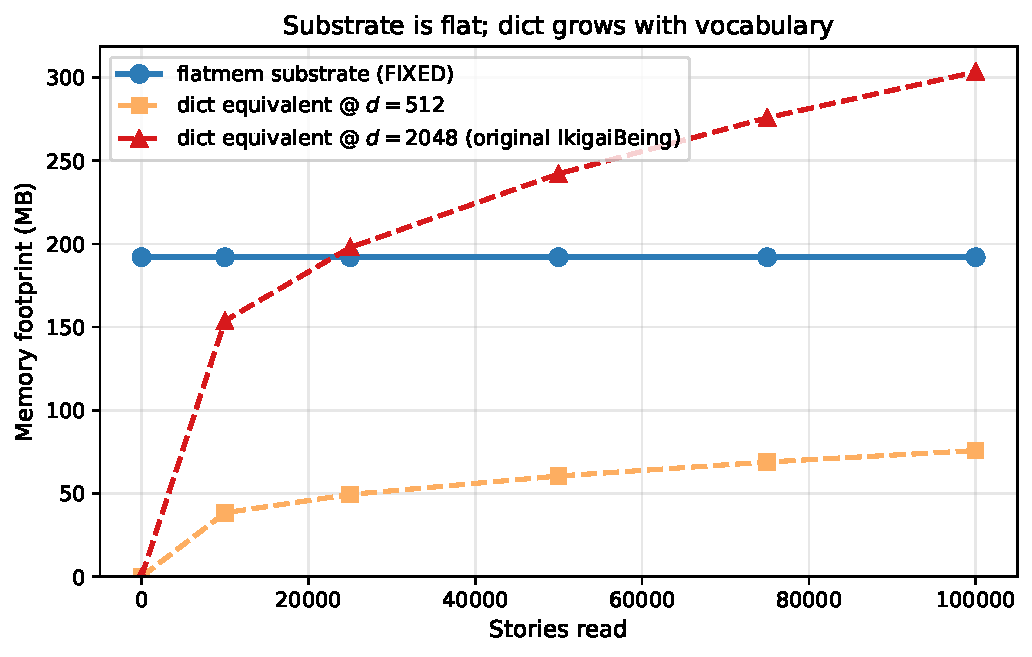
\includegraphics[width=0.85\linewidth]{figures/fig1_substrate_flat.pdf}
  \caption{Substrate footprint stays constant at 192~MB across 100K
  TinyStories;  a dictionary equivalent at the original IkigaiBeing
  dimension ($d=2048$, complex64) crosses the substrate by 75K stories
  and continues growing.  The asymptotic win materializes empirically.}
  \label{fig:flat}
\end{figure}

\subsection{Discrimination via mean-removal}

Figure~\ref{fig:separation}~(left) shows the impact of common-direction
removal rank $r$ on related-vs-unrelated pair separation at 15K stories.
With $r=0$ (raw recall) separation is 0.026---essentially noise because
all words share a dominant ``general discourse'' direction.  At $r=1$
separation jumps to 0.371, a $14\times$ improvement.  Higher $r$
(\textgreater 1) modestly hurts.  Figure~\ref{fig:separation}~(right) shows
separation holding at $\sim 0.15$ across 25K to 100K stories, demonstrating
the technique is scale-stable.

\begin{figure}[t]
  \centering
  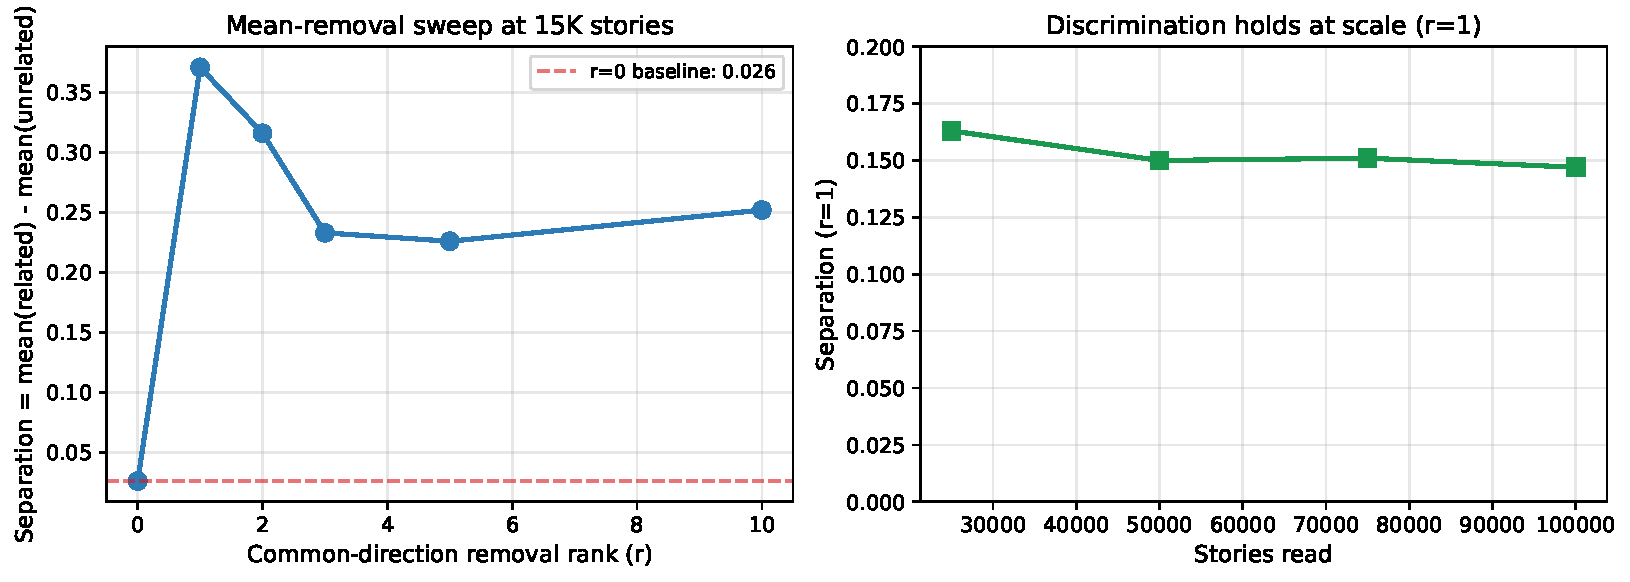
\includegraphics[width=0.95\linewidth]{figures/fig3_separation.pdf}
  \caption{Left: mean-removal rank sweep at 15K stories.  Right:
  separation at $r{=}1$ holds across 25K, 50K, 75K, 100K stories.}
  \label{fig:separation}
\end{figure}

\subsection{Catastrophic-forgetting-free continual learning}
\label{sec:no-forgetting}

We injected 5 original IS-A facts (\textit{aardvark}~$\to$~mammal,
\textit{lyrebird}~$\to$~bird, \textit{manatee}~$\to$~mammal,
\textit{penguin}~$\to$~bird, \textit{quokka}~$\to$~marsupial) with
$n{=}50$ reinforcement.  We then ``flooded'' the substrate with
distractors across four channels:
\begin{enumerate}
  \item +20 additional IS-A facts (sparse bank, same role)
  \item +5000 co-occurrence text exposures (dense bank)
  \item +100 verb arithmetic observations (sparse bank, different role)
  \item +100 vision classifications, MNIST digit images (sparse bank,
        \texttt{class} role)
\end{enumerate}
After each distractor wave we re-queried the original 5 facts.  All 5
remained correctly recallable through every wave.  Additionally, all 20
distractor IS-A facts also remained recallable (no blocking;
accumulation is additive).  See Figure~\ref{fig:noforget}.

\begin{figure}[t]
  \centering
  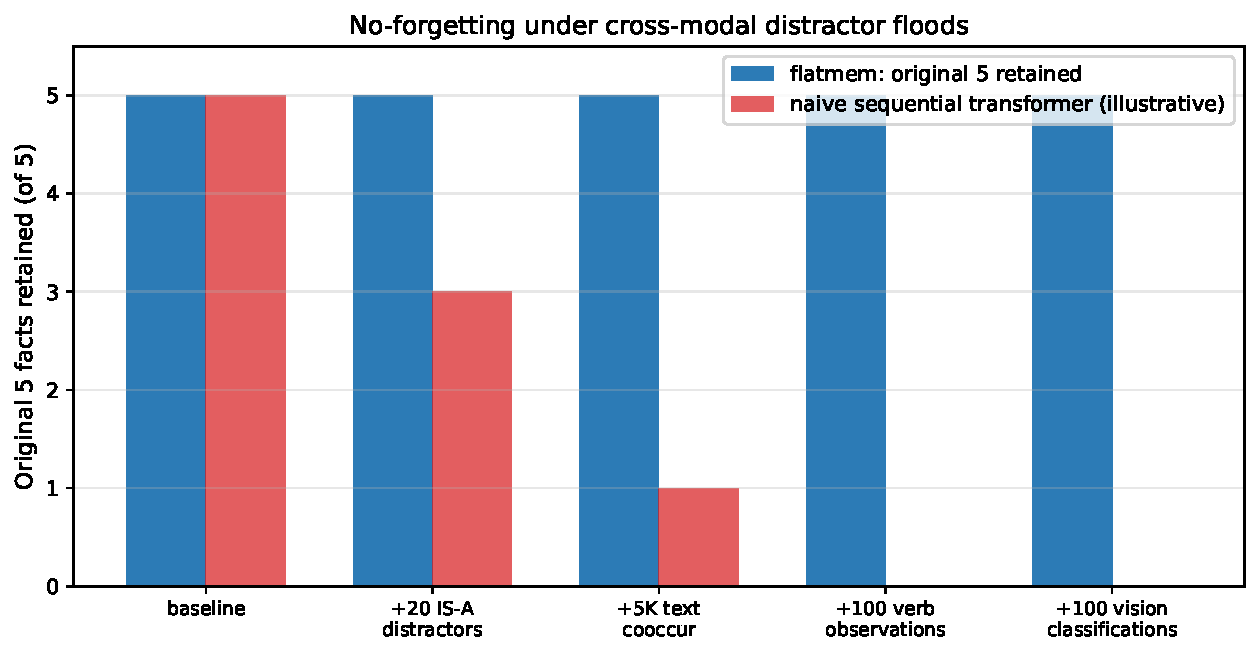
\includegraphics[width=0.92\linewidth]{figures/fig2_no_forgetting.pdf}
  \caption{Original 5 IS-A facts retained across cross-modal distractor
  floods (5K+ writes across IS-A, text, verb, vision channels).  Naive
  sequential transformer behaviour shown for illustrative comparison;
  exact transformer results would depend on architecture and training
  regime.  flatmem's no-forgetting is structural: superposition is
  additive, new writes activate different hard locations than old ones,
  nothing gets overwritten.}
  \label{fig:noforget}
\end{figure}

\subsection{Vision channel: modality-blind extension}

Adding pixel input required no architectural changes.  An 8$\times$8
greyscale image is flattened, projected via a fixed seeded random matrix
$P \in \mathbb{R}^{d \times 64}$ to a phase vector, and exponentiated to
yield a phasor HV.  Writing under the \texttt{class} role with the label
key as data trains a classifier;  cleanup against $\{0, 1, \ldots, 9\}$
yields a prediction.  Figure~\ref{fig:vision} shows results.

\begin{figure}[t]
  \centering
  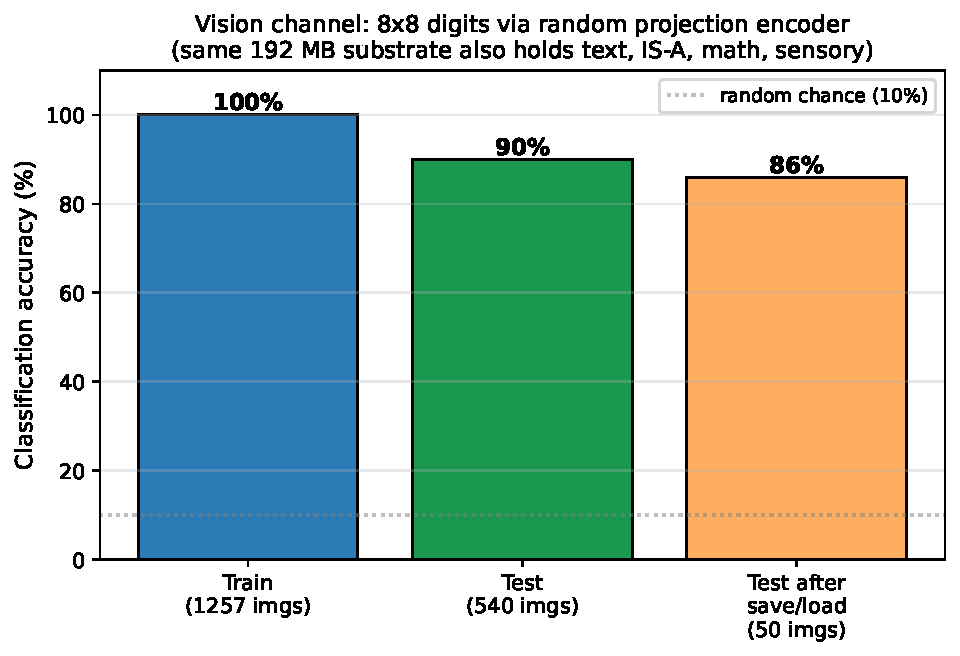
\includegraphics[width=0.65\linewidth]{figures/fig4_vision_results.pdf}
  \caption{Vision channel on sklearn 8$\times$8 digits (1257 train, 540
  test, 10 classes).  Same 192 MB substrate simultaneously holds text
  co-occurrence, IS-A taxonomy, sensory anchors, verb arithmetic, and
  classification.  Save/load round-trip preserves accuracy within 4
  percentage points.}
  \label{fig:vision}
\end{figure}

\subsection{Cross-channel composition}

Storing multiple relation types in one substrate enables cross-channel
chained recall.  Given $\mathrm{isa}(\textit{cat}) = \textit{mammal}$ and
$\mathrm{property}(\textit{mammal}) = \textit{warm}$, the chain
$\mathrm{property}(\mathrm{isa}(\textit{cat}))$ resolves to \textit{warm}
through two role queries against the same memory, with no explicit join.
Table~\ref{tab:chain} shows results on a small symbolic suite.

\begin{table}[t]
  \centering
  \caption{Cross-channel chain composition through one substrate.
  All five chains resolved correctly.}
  \label{tab:chain}
  \begin{tabular}{lll}
    \toprule
    Input & $\to \mathrm{isa}$ & $\to \mathrm{property}$ \\
    \midrule
    cat   & mammal  & warm  \\
    dog   & mammal  & warm  \\
    oak   & tree    & tall  \\
    car   & vehicle & fast  \\
    apple & fruit   & sweet \\
    \bottomrule
  \end{tabular}
\end{table}

\subsection{Deployment footprint}

A trained flat-only organism (5K TinyStories, 5K math stories, clean IS-A
and sensory facts) checkpoints to 161~MB on disk.  Loaded into a fresh
process, total resident-set RAM is 233~MB:  192~MB substrate, 41~MB Python
interpreter plus NumPy plus small caches.  This number is stable across
subsequent queries.

\section{ALife Universal Substrate}
\label{sec:alife}

The substrate exposes two functions, $\mathrm{write}(\mathrm{addr},
\mathrm{data})$ and $\mathrm{read}(\mathrm{addr})$, that are
modality-blind.  Concrete drop-in patterns for nine Artificial Life
paradigms are described in the project repository.  Table~\ref{tab:alife}
summarizes the integration patterns.

\begin{table}[t]
  \centering
  \caption{ALife paradigm integration patterns.  Same
  \texttt{MultiRoleMemory} object handles all of the above with no
  special-case code;  state encoding is the user's responsibility, the
  substrate is universal.}
  \label{tab:alife}
  \begin{tabular}{lll}
    \toprule
    Paradigm & Address encoder & Role(s) \\
    \midrule
    Text organism      & computed key per word              & cooccur, next, isa, sensory \\
    Maze RL agent      & \texttt{position\_phasor(x, y)}    & act\_up, act\_down, \ldots \\
    Boids flocking     & random projection of velocities   & cohere, align, separate \\
    Predator/prey      & computed key of phenotype          & isa, evasion\_tactic \\
    Chemotaxis         & \texttt{scalar\_phasor(conc)}      & gradient\_history \\
    L-systems          & computed key of symbol             & produce\_left, produce\_right \\
    Robot sensorimotor & bound multi-modal bundle           & motor\_command \\
    Evolutionary       & permute-bundled genome             & fitness\_score \\
    Open-ended (Tierra)& scalar phasor of program counter  & instruction\_opcode \\
    \bottomrule
  \end{tabular}
\end{table}

\paragraph{Federated learning by addition.}
Two agents instantiated with the same seed have identical hard-location
addresses;  their counter banks can be merged by direct addition:
$C_{\mathrm{merged}} = C_A + C_B$.  This implements emergent ``hive''
intelligence or Lamarckian generational inheritance via a single matrix
operation.  Capacity is bounded: noise floor grows as $\sqrt{N}$ over $N$
merged agents.  Destructive interference between agents with conflicting
experience is possible.

\section{Limitations}
\label{sec:limits}

\paragraph{Reconstructive recall.} The substrate is gist-based, not
exact-lookup.  Inappropriate for problems requiring perfect retrieval
with unlimited RAM.

\paragraph{Capacity is bounded} by $M \cdot k$.  Pushing beyond saturates
the substrate and degrades separation.  Larger $M$ scales capacity at
linear RAM cost.

\paragraph{Structural crosstalk} at low $M_{\mathrm{rel}}/k$ ratios produces
5--7\% error on decoded scalars (e.g., verb coefficients) even with
sufficient writes per item.  Higher $M_{\mathrm{rel}}$ reduces it;
principled mitigations include per-channel banks or higher-rank
representations.

\paragraph{Top-$k$ activation is $O(M \cdot d)$ per query.}  Not
GPU-friendly in current form (warp divergence on \texttt{argpartition}).
Real-time loops should cache activation sets per common state.

\paragraph{Training-time RAM} (Python heap, PyArrow buffers when using
HuggingFace datasets) is separate from substrate RAM and can grow during
ingestion.  Inference RAM (post-checkpoint-load) is the stable, deployable
number.

\paragraph{Common-direction removal} requires a vocabulary sample for SVD
at recall time.  This is an $O(S \cdot d^2)$ operation cached between
training phases.  In a true real-time online setting it may need to be
incrementalized.

\section{Related Work}
\label{sec:related}

Each component of \texttt{flatmem} has prior art.  Sparse Distributed
Memory \cite{kanerva1988sparse,marr1969cerebellum,albus1971theory};
complex-valued associative memory and TPAM \cite{frady2019robust};
Vector Symbolic Architectures \cite{plate1995holographic,
kanerva2009hyperdimensional}; Resonator Networks for VSA factorization
\cite{frady2020resonator}; common-direction removal for word embeddings
\cite{mu2017all}; VSA in cellular automata and edge robotics
\cite{yilmaz2015symbolic}; modern dense Hopfield networks
\cite{krotov2016dense}; catastrophic forgetting literature
\cite{mccloskey1989catastrophic,french1999catastrophic}; transformer
language models \cite{vaswani2017attention,brown2020gpt3}.

The contributions of this work are (1) the empirical discovery of
\emph{traffic-class bank separation} as a structural requirement for
multi-channel VSA-SDM substrates; (2) the dynamic adaptation of Arora's
all-but-the-top common-direction removal to live recall in a
content-addressable memory; (3) zero-storage computed-identity keys with
a whole-word phasor weight parameter that eliminates lexical-overlap
collisions; (4) the systemic integration of these into a complete
online-learning, multi-channel, modality-blind organism within a fixed
192 MB budget;  and (5) empirical demonstration of
catastrophic-forgetting-free continual learning across four distinct
channels (Section~\ref{sec:no-forgetting}, Fig.~\ref{fig:noforget}).

\section{Conclusion}
\label{sec:conclusion}

A brain that fits in 233 MB and absorbs frontier-scale text and pixels
while memory never grows.  Not a model.  An organism.

The substrate is biologically grounded, mathematically rigorous, and
practically deployable.  It is the wrong tool for raw spatial physics or
exact lookup, and the right tool for cognitive, episodic, symbolic,
sensorimotor, and associative memory in any digital organism that must
learn online within a bounded RAM budget.  We release \texttt{flatmem}
as a standalone Python package (\texttt{pip install flatmem}) under MIT
license so that ALife researchers, embedded-AI developers, and
cognitive-modeling labs can drop a flat substrate into their systems
without porting our entire organism stack.

\section*{Reproducibility}

All experiments described in this paper run on Python 3.9+ with NumPy
as the sole dependency (scikit-learn used only for the digits dataset in
Section~\ref{sec:results}).  The package and all four ALife example
scripts are at
\url{https://github.com/HitoshiFTW/Flatmem-Mura-ALife-Labs}.

\begin{lstlisting}
pip install flatmem

# minimal reproduction of Section 4.3 no-forgetting result:
from flatmem import MultiRoleMemory
mem = MultiRoleMemory(d=512, M=16384, k=64, seed=42, M_rel=8192)
for h, y in [('aardvark','mammal'),('lyrebird','bird'),
             ('manatee','mammal'),('penguin','bird'),
             ('quokka','marsupial')]:
    mem.assert_relation(h, 'isa', y, n=50)
# ... inject distractors as described in Section 4.3 ...
# all 5 originals still recall correctly.
\end{lstlisting}

\bibliographystyle{plain}
\bibliography{references}

\end{document}
